\documentclass[12pt]{article}

% Misc. packages
\usepackage{array,calc,lastpage}
\usepackage{amsmath,amssymb}
\usepackage{graphicx,subfig,rotating,placeins}

% Page layout
\usepackage[left=10mm, right=10mm, top=20mm, bottom=20mm]{geometry}
\flushbottom

% Headers and footers
\usepackage{fancyhdr}
\pagestyle{fancy}
\lhead{{The East Scarborough Storefront Calendar User Manual}}
\chead{{}}
\rhead{{}}
\lfoot{{}}
\cfoot{{}}
\rfoot{{Page \thepage\ of \pageref{LastPage}}}

% Sectioning commands
\usepackage{titlesec}
\titleformat{\section}{\large\bfseries}{\thesection}{1em}{}

% Paragraph style
\raggedright 
\setlength{\parindent}{0pt}
\setlength{\parskip}{8pt}

\title{The East Scarborough Storefront Calendar User Manual}
\date{November 2013}
\author{Developed by CSC301H1 Team Nettilling:\\H. Chen, S. Dao, M. Haber, Y. Khvan, T. Letchumanan, J.P. McCool\\Department of Computer Science\\The University of Toronto St. George}



\begin{document}

\maketitle              \newpage
\section*{Introduction}


\subsection*{What is the Storefront Calendar?}

The Storefront Calendar is a web-based tool used to book Storefront spaces.


\subsection*{Who may use the Calendar?}

Storefront administrators, front-desk staff, and designated Storefront partner-agents.


\subsection*{Where can I access the Calendar?}

You can access the Storefront Calendar at this web-address: http://thestorefront.cloudapp.net/

For best results, it is recommended that you use either Mozilla Firefox or Google Chrome as your web-browser.


\subsection*{How can I get a Calendar account?}

If you are a Storefront administrator, you have already been assigned a Calendar ID and password.

If you are a front-desk staff member, you should use the staff ID and password provided by the administration.

If you are a Storefront partner, and do not have a Calendar account (and want one), please contact the Storefront at:\newline\newline
\begin{tabular}{l l}
Phone: & (416) 208-9889 \\
Fax:   & (416) 208-9239 \\
\end{tabular}


\subsection*{How do I use the Calendar website?}

That's the topic of this manual!






        \newpage
\tableofcontents        \newpage
\section{The Basics}

The Storefront Calendar is located at: http://thestorefront.cloudapp.net/


\subsection{Logging In}

Enter your username and password in the indicated fields of the ``LOGIN'' box, then click the ``Log in'' button.

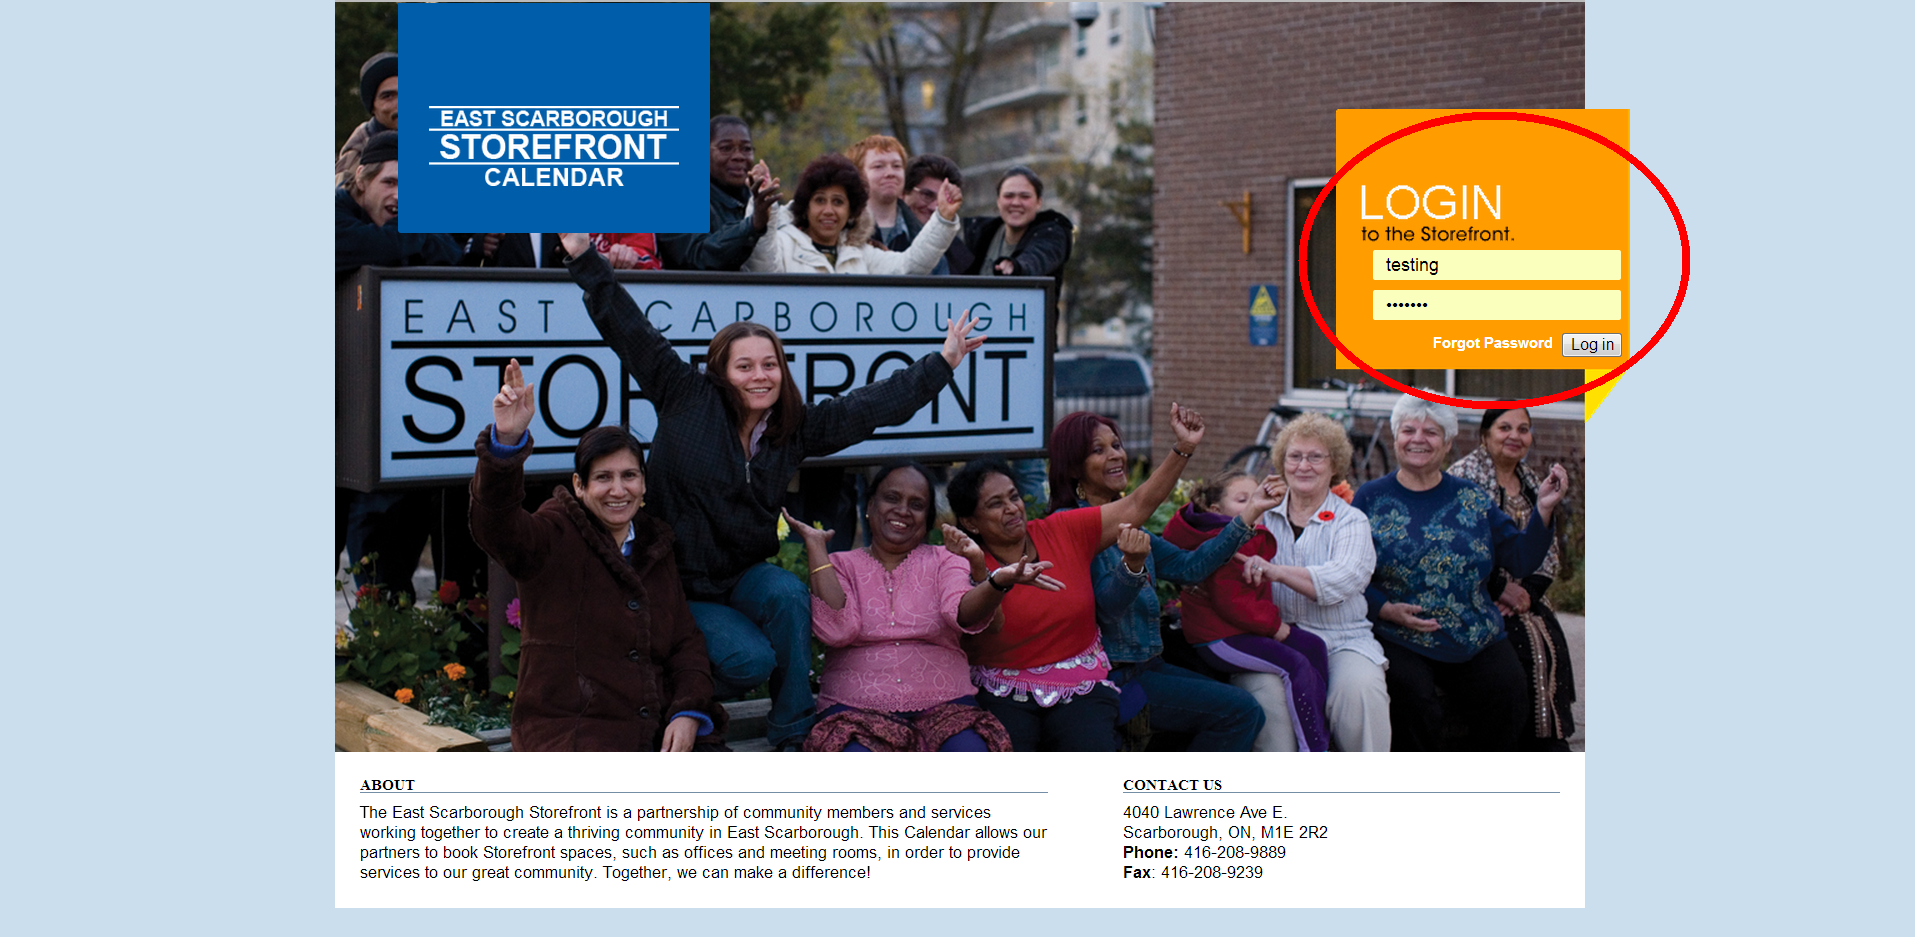
\includegraphics[width=\linewidth]{screenshots/img_login}


\newpage



\subsection{Logging Out}

You can log out of the website by clicking the ``Logout'' button in the upper-right corner of the main view.

To prevent others from accessing your account, it is recommended that you log out whenever you are not using the Calendar.

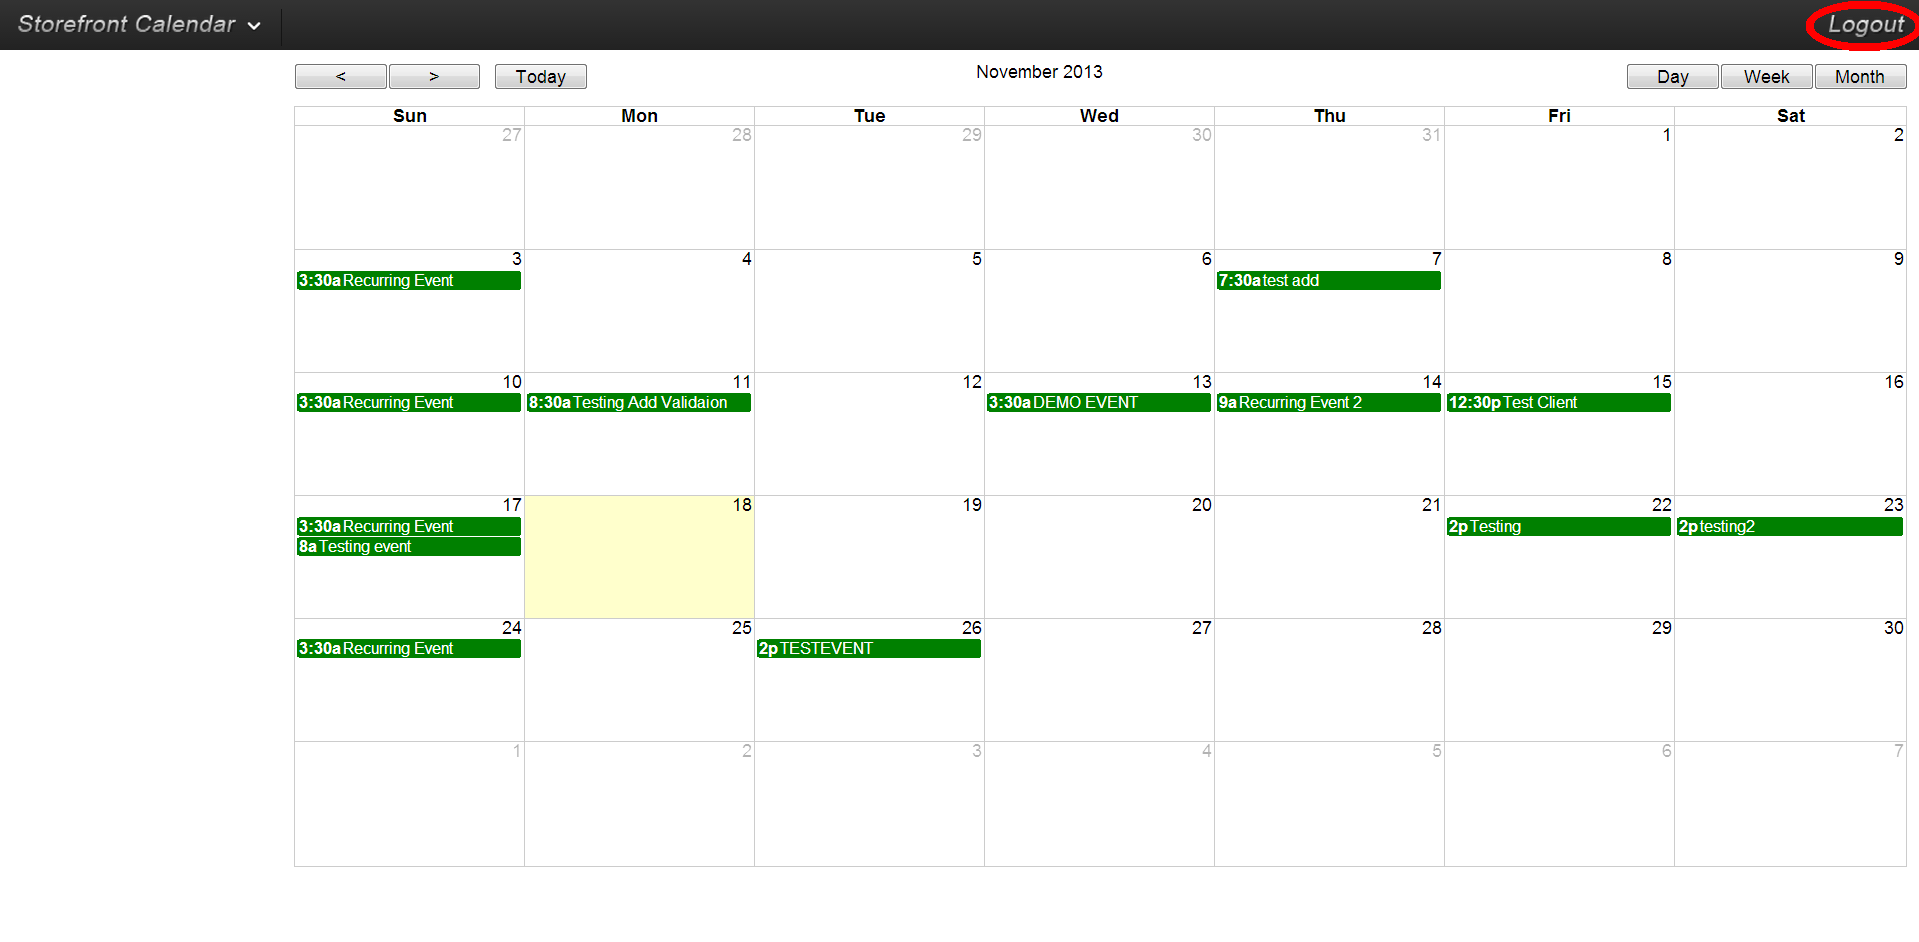
\includegraphics[width=\linewidth]{screenshots/img_logout}


       \newpage
\section{Getting Around -- Site Navigation}

After logging in (and performing most actions), you will be presented with a calendar view of the current month's events.

There are three different ways to see the currently booked events: by month, by week, and by day. You can switch between each view by clicking the buttons in the upper-right hand corner of the screen.


\subsection{Events}

Events are room bookings made in the name of a Storefront Partner. Events are colour coded according to their status: tentative (blue), confirmed (green), or rejected (red). Only Administrator-level users can make confirmed bookings, or change booking statuses. All other user levels may only create tentative (requested) events.


\subsection{Navigation by Month}

This is the default view that you will see after logging in. By default, the month presented is the current month. To view a different month, navigate backwards and forwards using the arrow buttons in the upper-left corner.

Tip: If you are an Administrator, you can drag-and-drop events to different days. You can also confirm a tentative booking by single left-clicking on it.

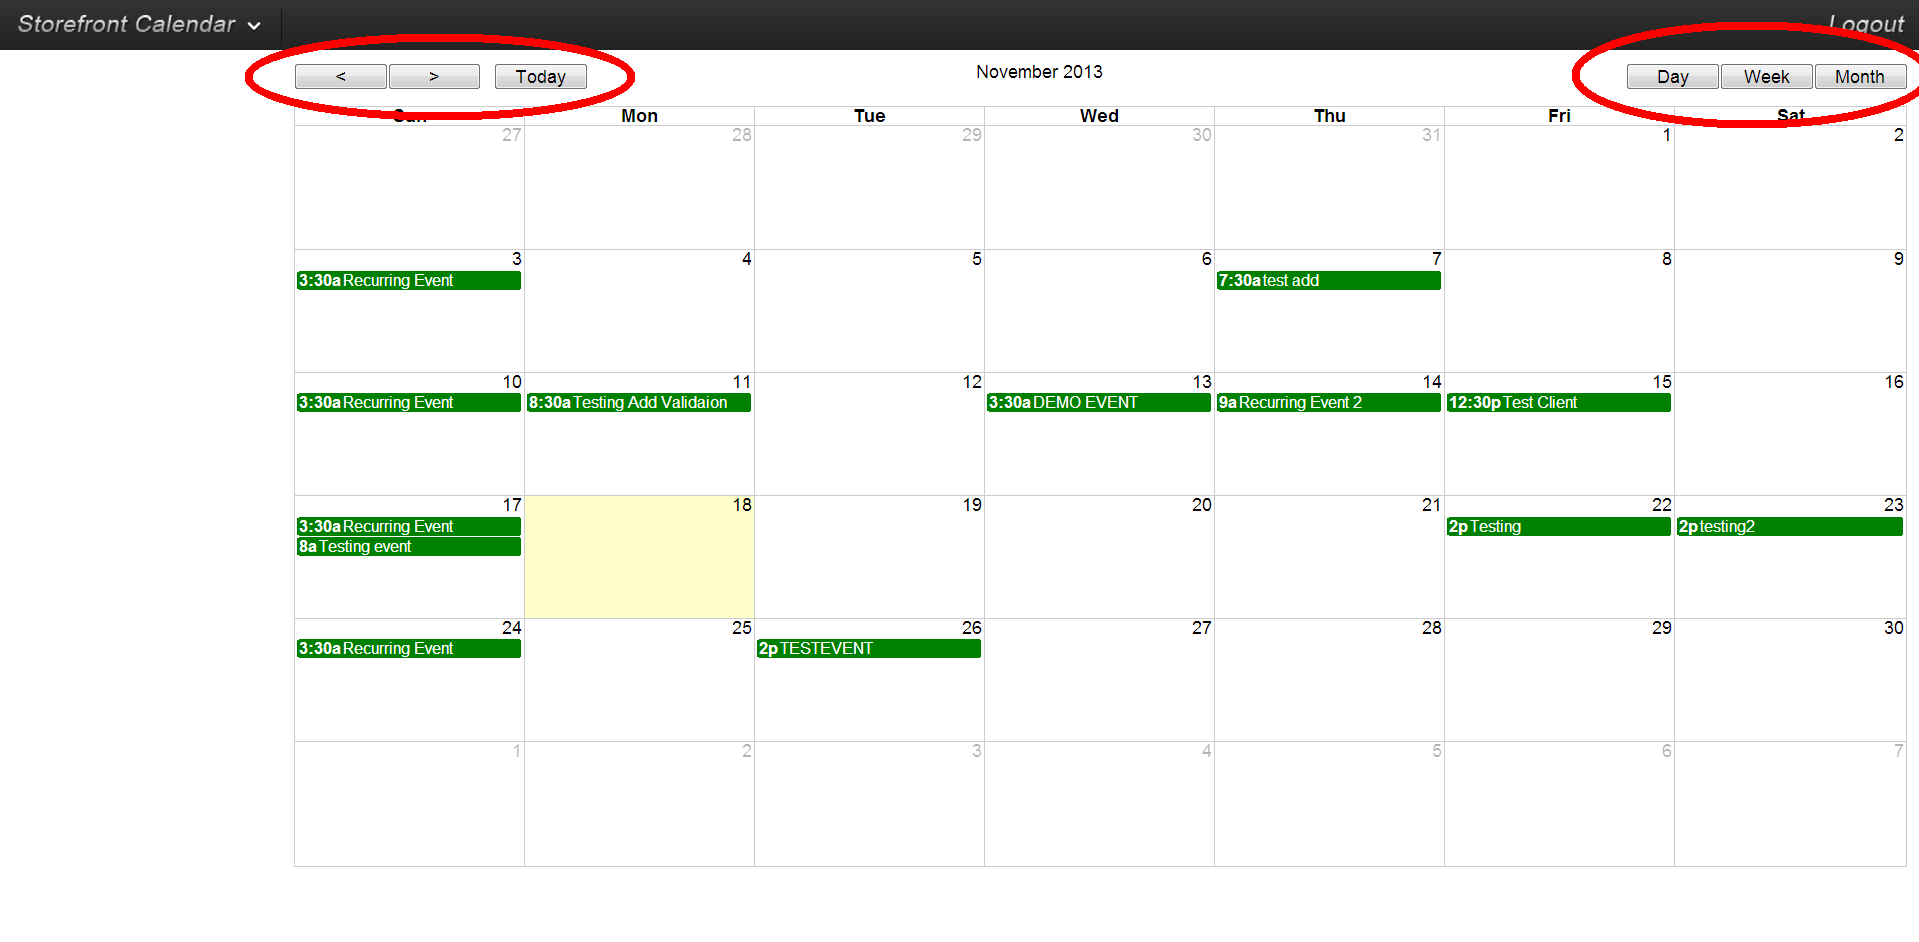
\includegraphics[width=\linewidth]{screenshots/img_month}

\newpage


\subsection{Navigation by Week}

In this view, the columns are days of the week, and the rows are booking times. By default, the week presented is the current week. To view a different week, navigate backwards and forwards using the arrow buttons.

Tip: If you are an Administrator, you can drag-and-drop events to different days and times. You can also confirm a tentative booking by single left-clicking on it.

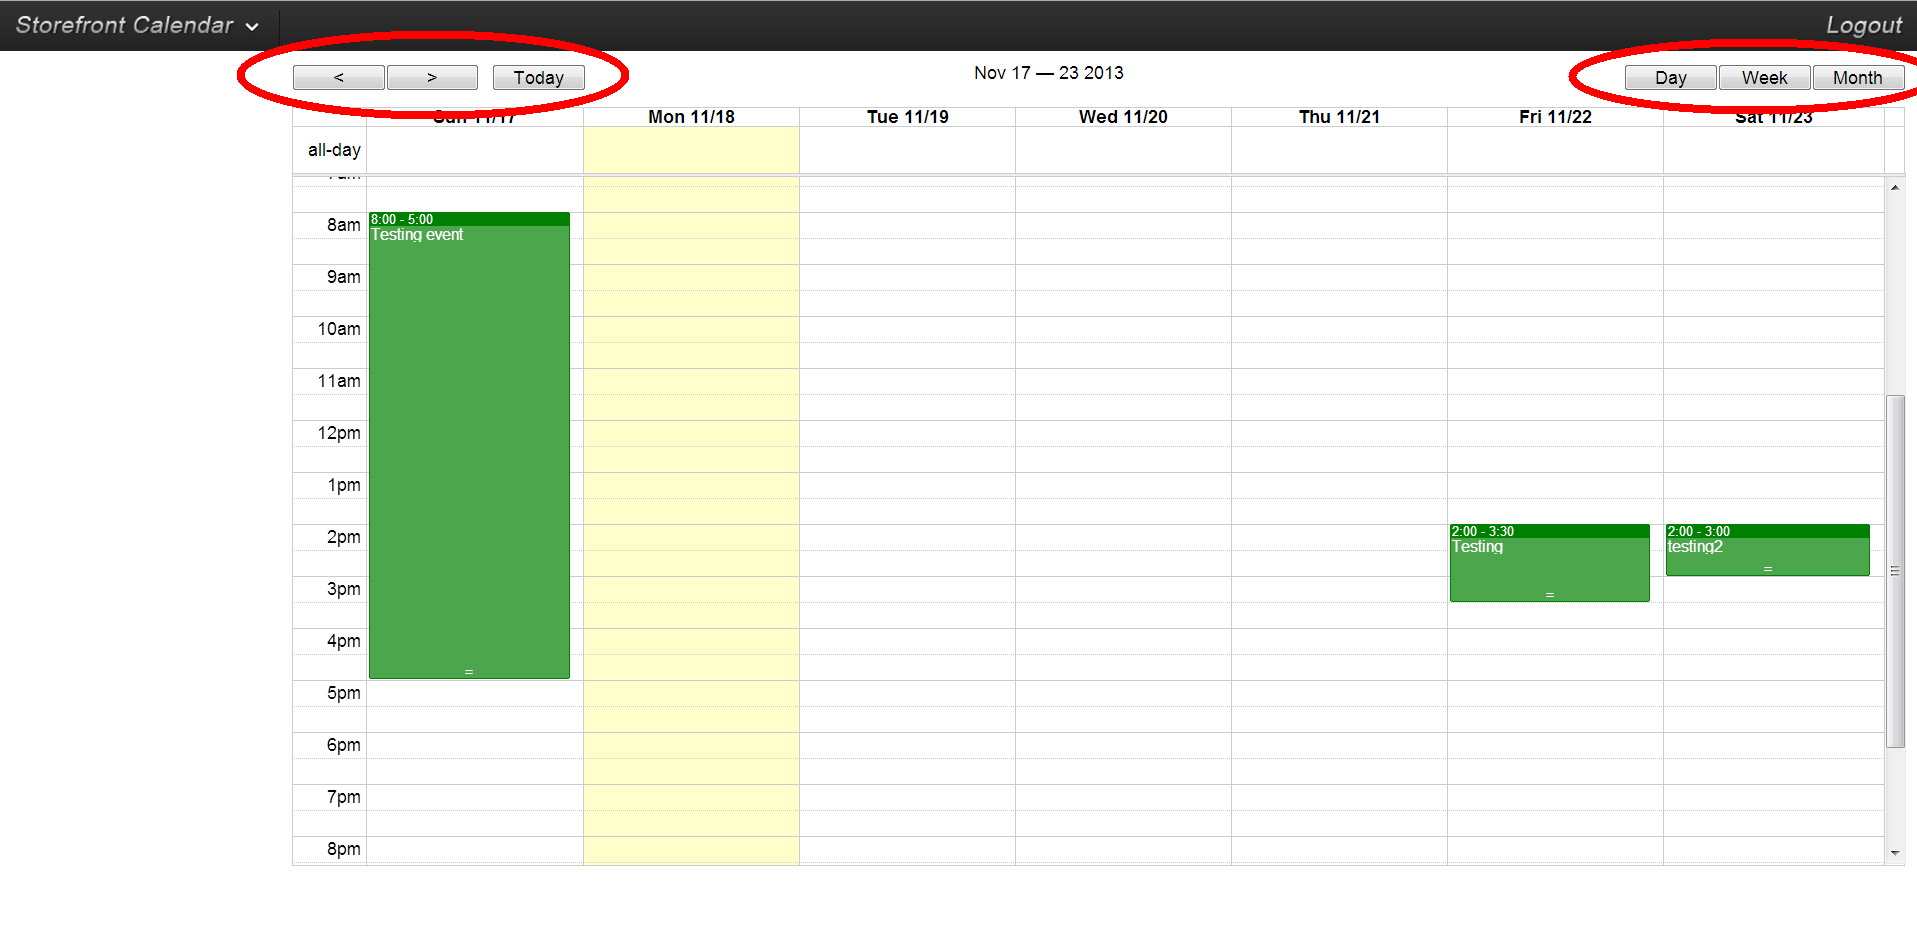
\includegraphics[width=\linewidth]{screenshots/img_week}


\newpage


\subsection{Navigation by Day}

The columns are bookable rooms, and the rows are booking times. By default, the day presented is the current day. To view a different day, navigate backwards and forwards using the arrow buttons.

Tip: If you are an Administrator, you can drag-and-drop events to different times and rooms. You can also confirm a tentative booking by single left-clicking on it.

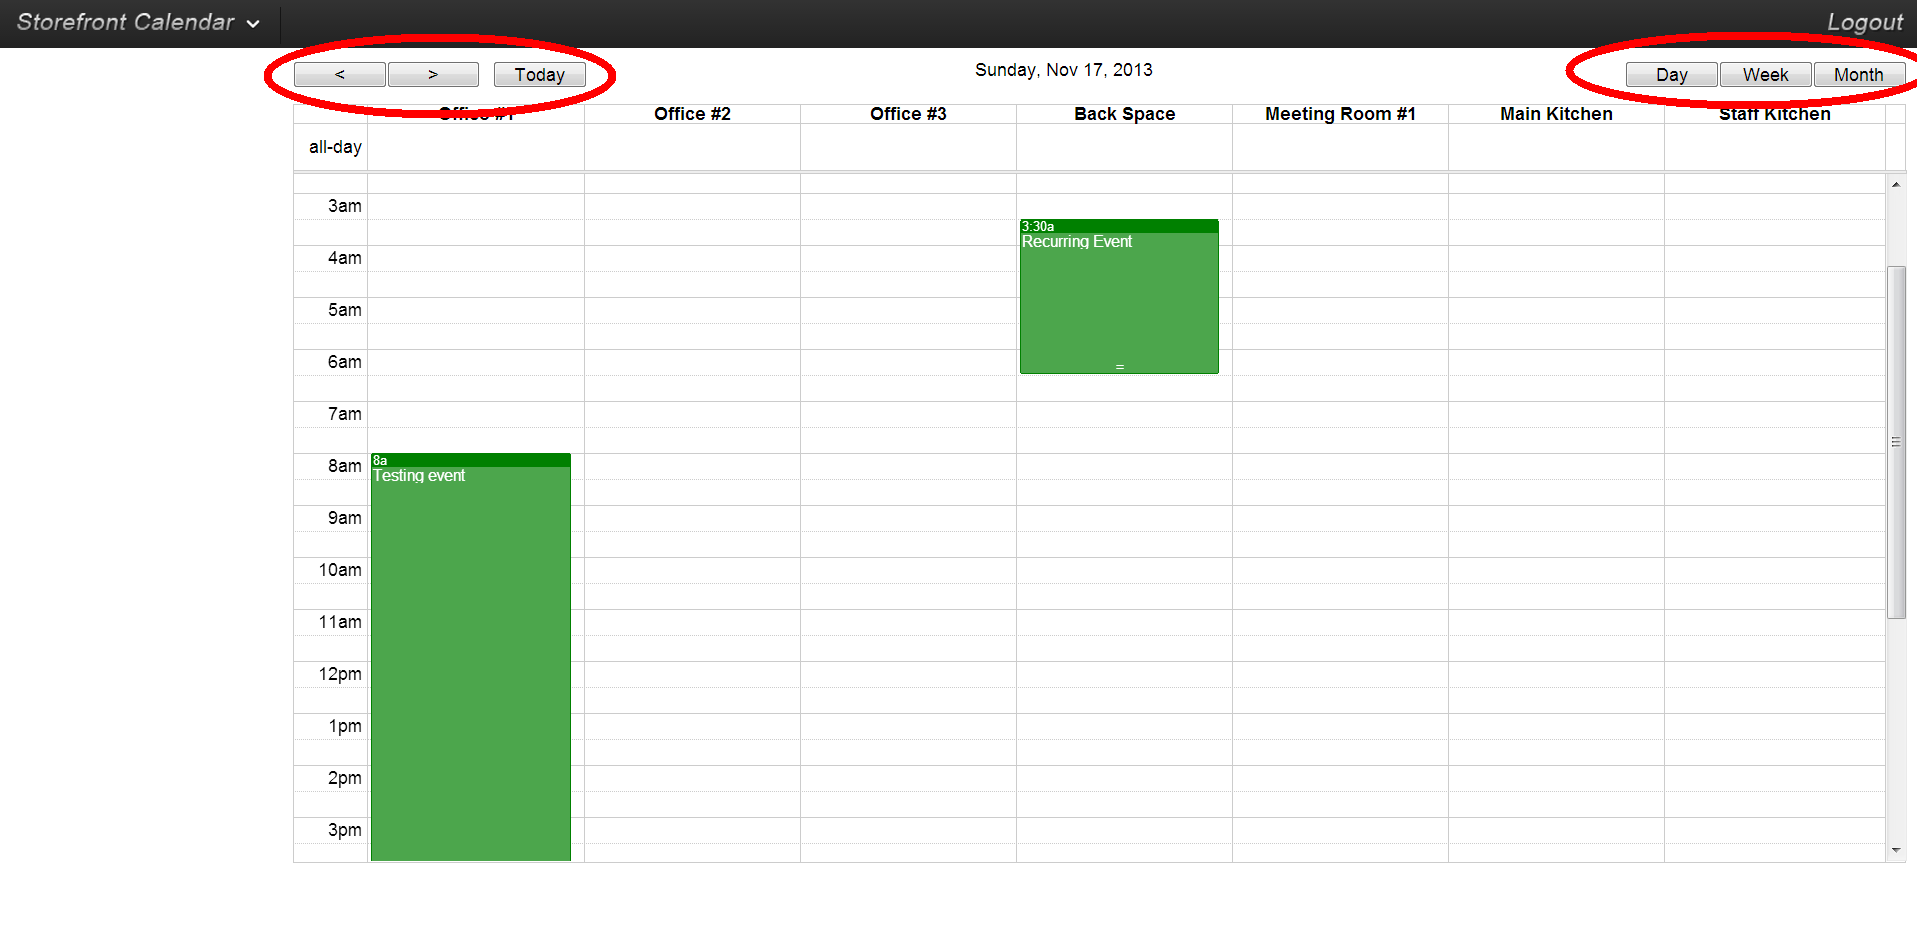
\includegraphics[width=\linewidth]{screenshots/img_day}



         \newpage
\section{Adding and Editing Events}


\subsection{Adding a New Event}

To add a new event to the system, select ``New Event'' from the drop-down menu in the Toolbar. You will be directed to the ``Add New Booking'' form. Fill out all the required fields in the form, and click ``Continue''. If you want to clear the form, click 'Reset'.

If you are not an Administrator, you may only add \textit{tentative} (\textit{requested}) events; an Administrator will need to confirm your room booking.

If you are an Administrator or a Staff member, you may add events on behalf of any Partner. If you are a Partner, you may add events only on your own organization's behalf.

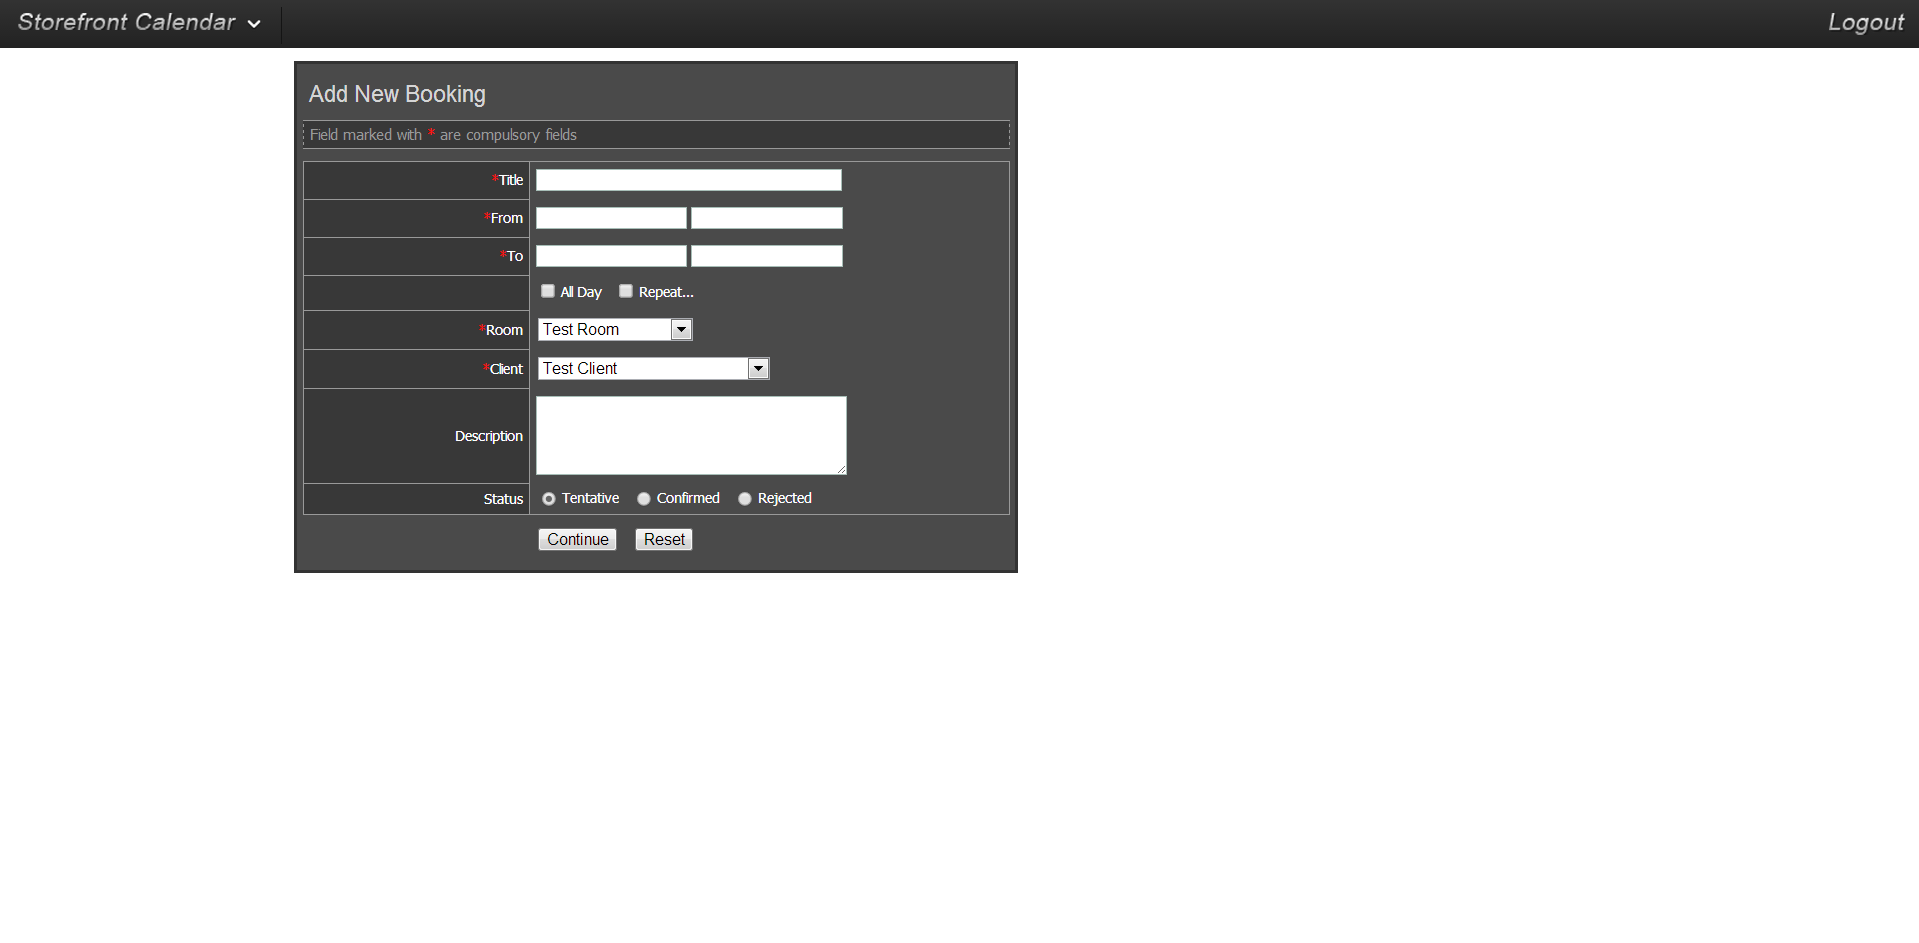
\includegraphics[width=\linewidth]{screenshots/img_addevent}

\newpage


\subsection{Editing an Existing Event}

To edit an existing event, select ``Edit Event'' from the drop-down menu in the Toolbar. You will be directed to the ``Edit Bookings'' form. Fill out all the required fields in the form, and click ``Save''. If you want to delete the event, click ``Delete''.

If you are not an Administrator and you edit a non-tentative booking, it will become tentative; an Administrator will need to confirm the new booking details.

If you are an Administrator or a Staff member, you may edit events on behalf of any Partner. If you are a Partner, you may edit only your own organization's events.

Shortcut: You can also edit an event by double left-clicking on it. If you are a Partner and do not own the event, the ``Edit Bookings'' form will still be brought up, however you will only be able to edit bookings you own.

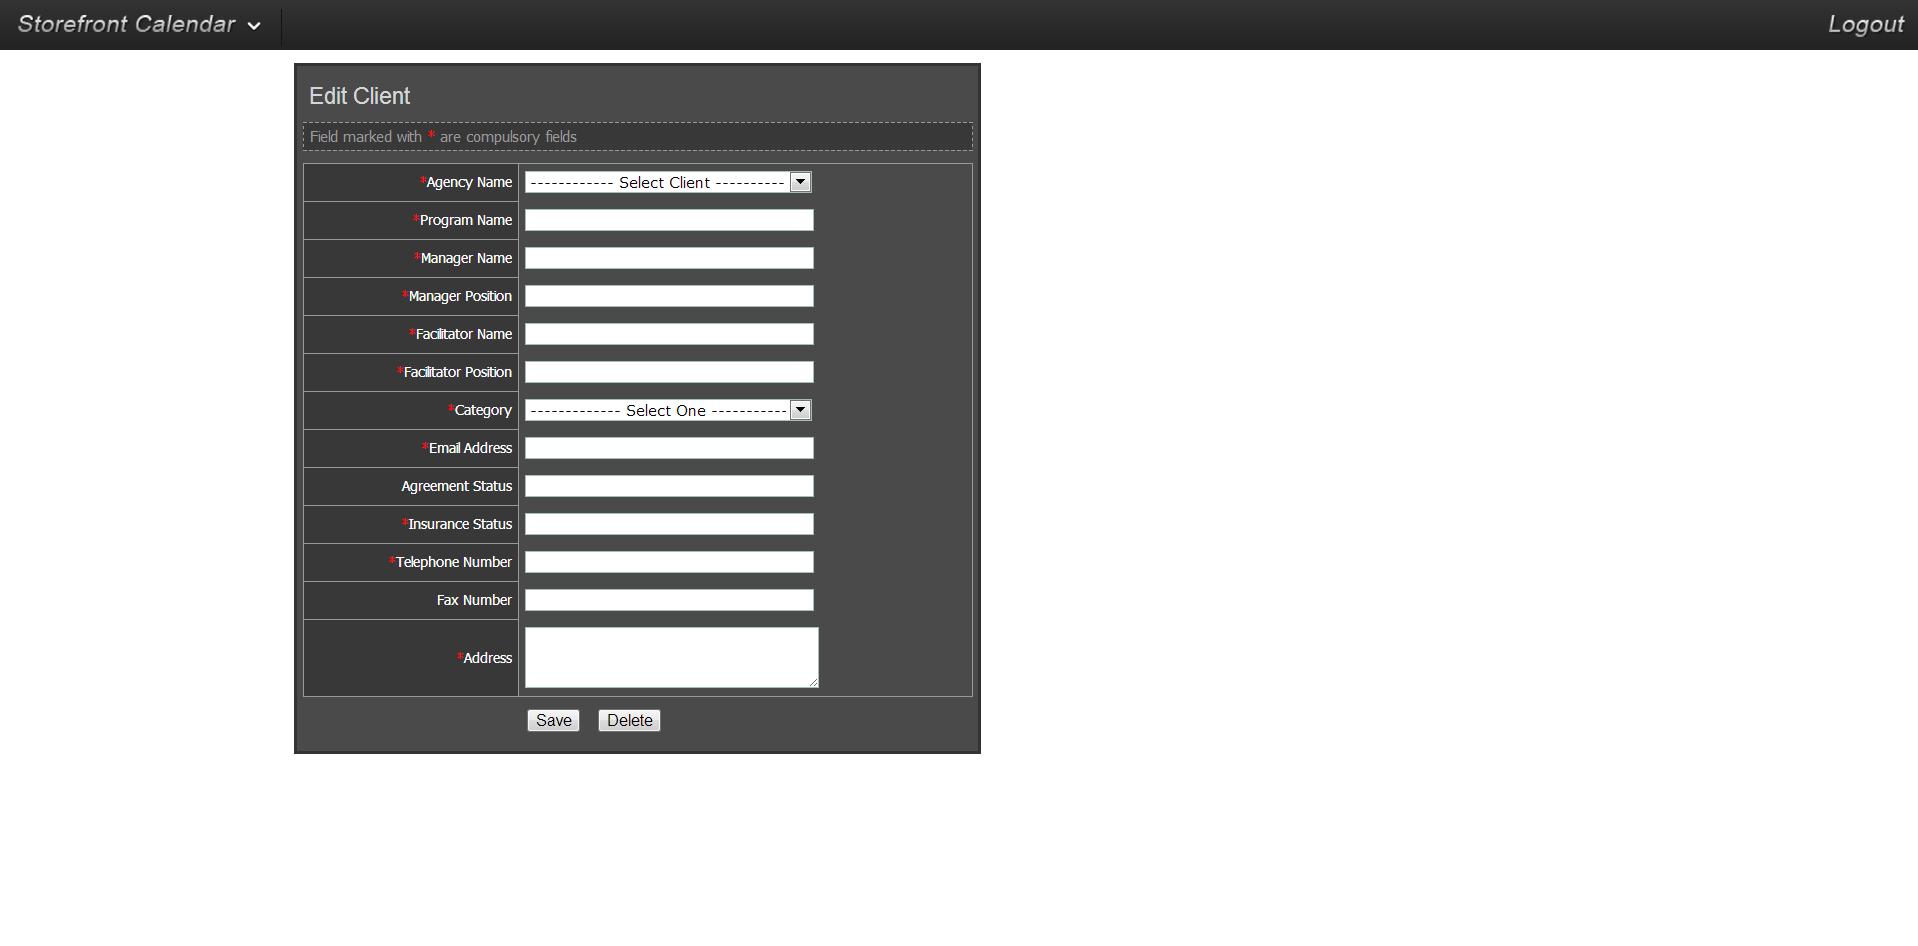
\includegraphics[width=\linewidth]{screenshots/img_editevent}

       \newpage
\section{Adding and Editing Users (Administrators Only)}

Only Administrators can add and edit user accounts.


\subsection{Adding a New User}

To add a new user to the system, select ``Add New User'' from the drop-down menu in the Toolbar. You will be directed to the ``Add New User'' form. Fill out all the required fields in the form, and click ``Continue''. If you want to clear the form, click 'Reset'.

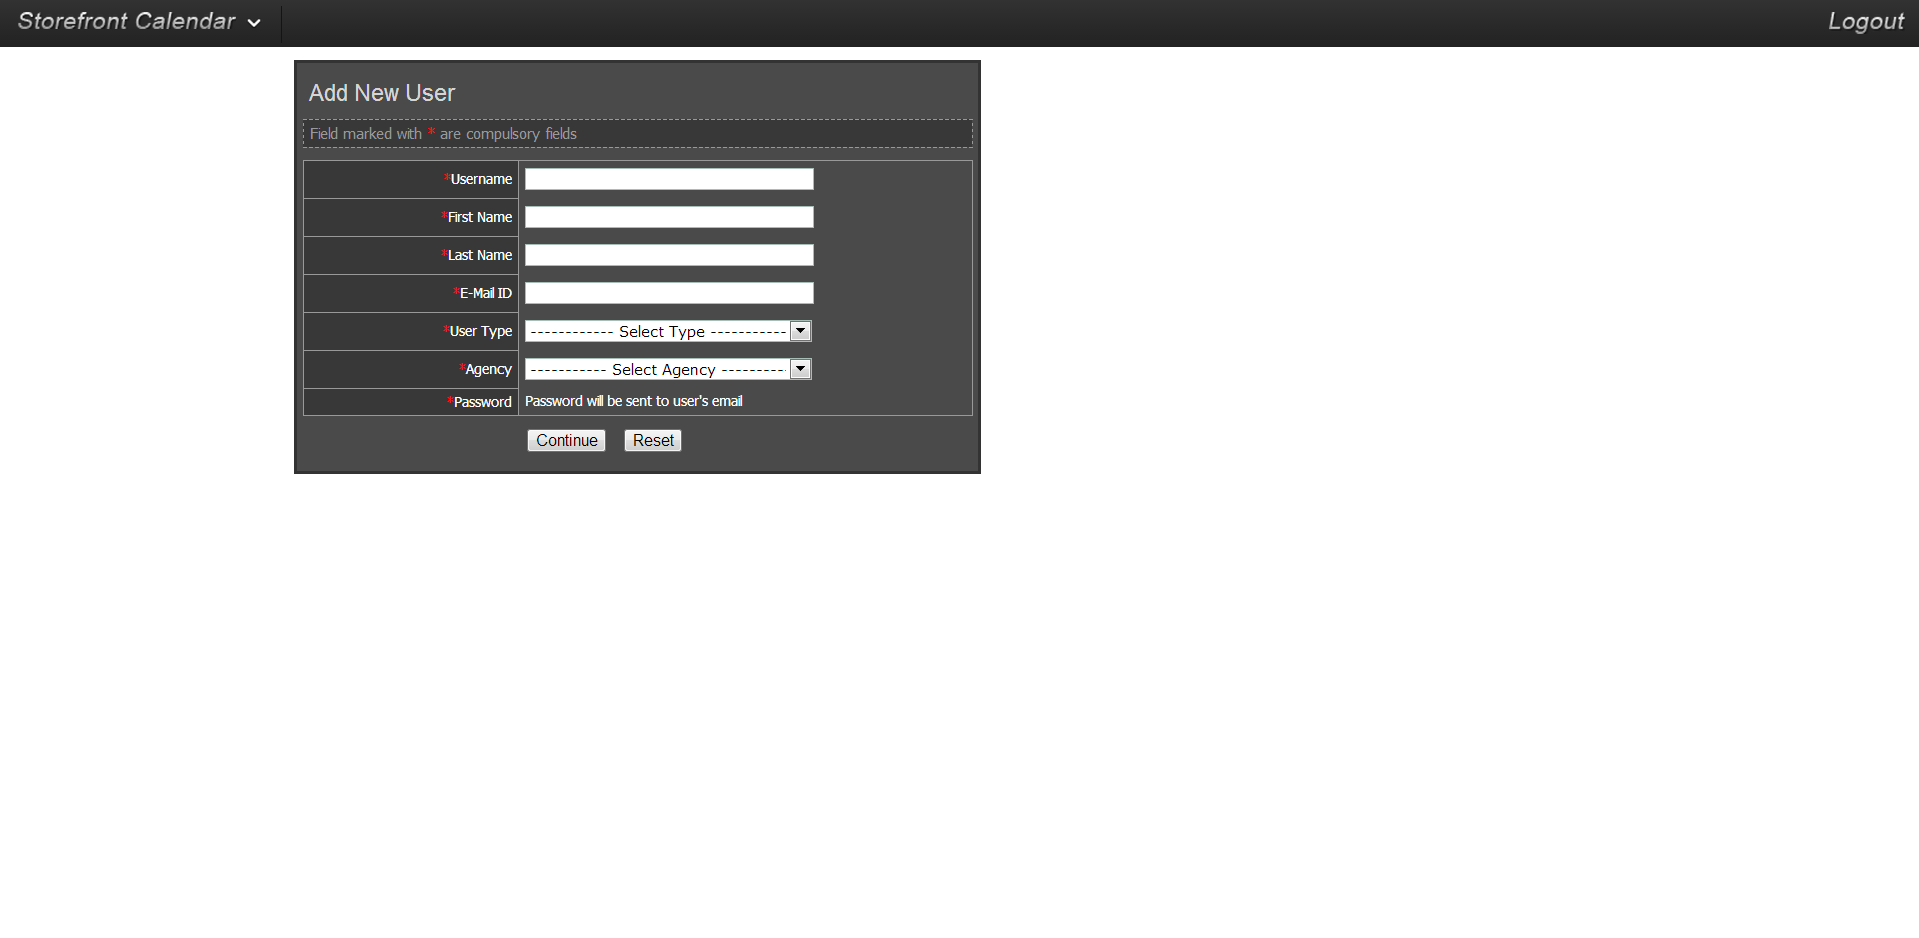
\includegraphics[width=\linewidth]{screenshots/img_adduser}


\newpage


\subsection{Editing an Existing User}

To edit an existing user, select ``Edit User'' from the drop-down menu in the Toolbar. You will be directed to the ``Edit User'' form. Fill out all the required fields in the form, and click ``Save''. If you want to delete the user, click ``Delete''. You cannot delete your own account, even as an Administrator.

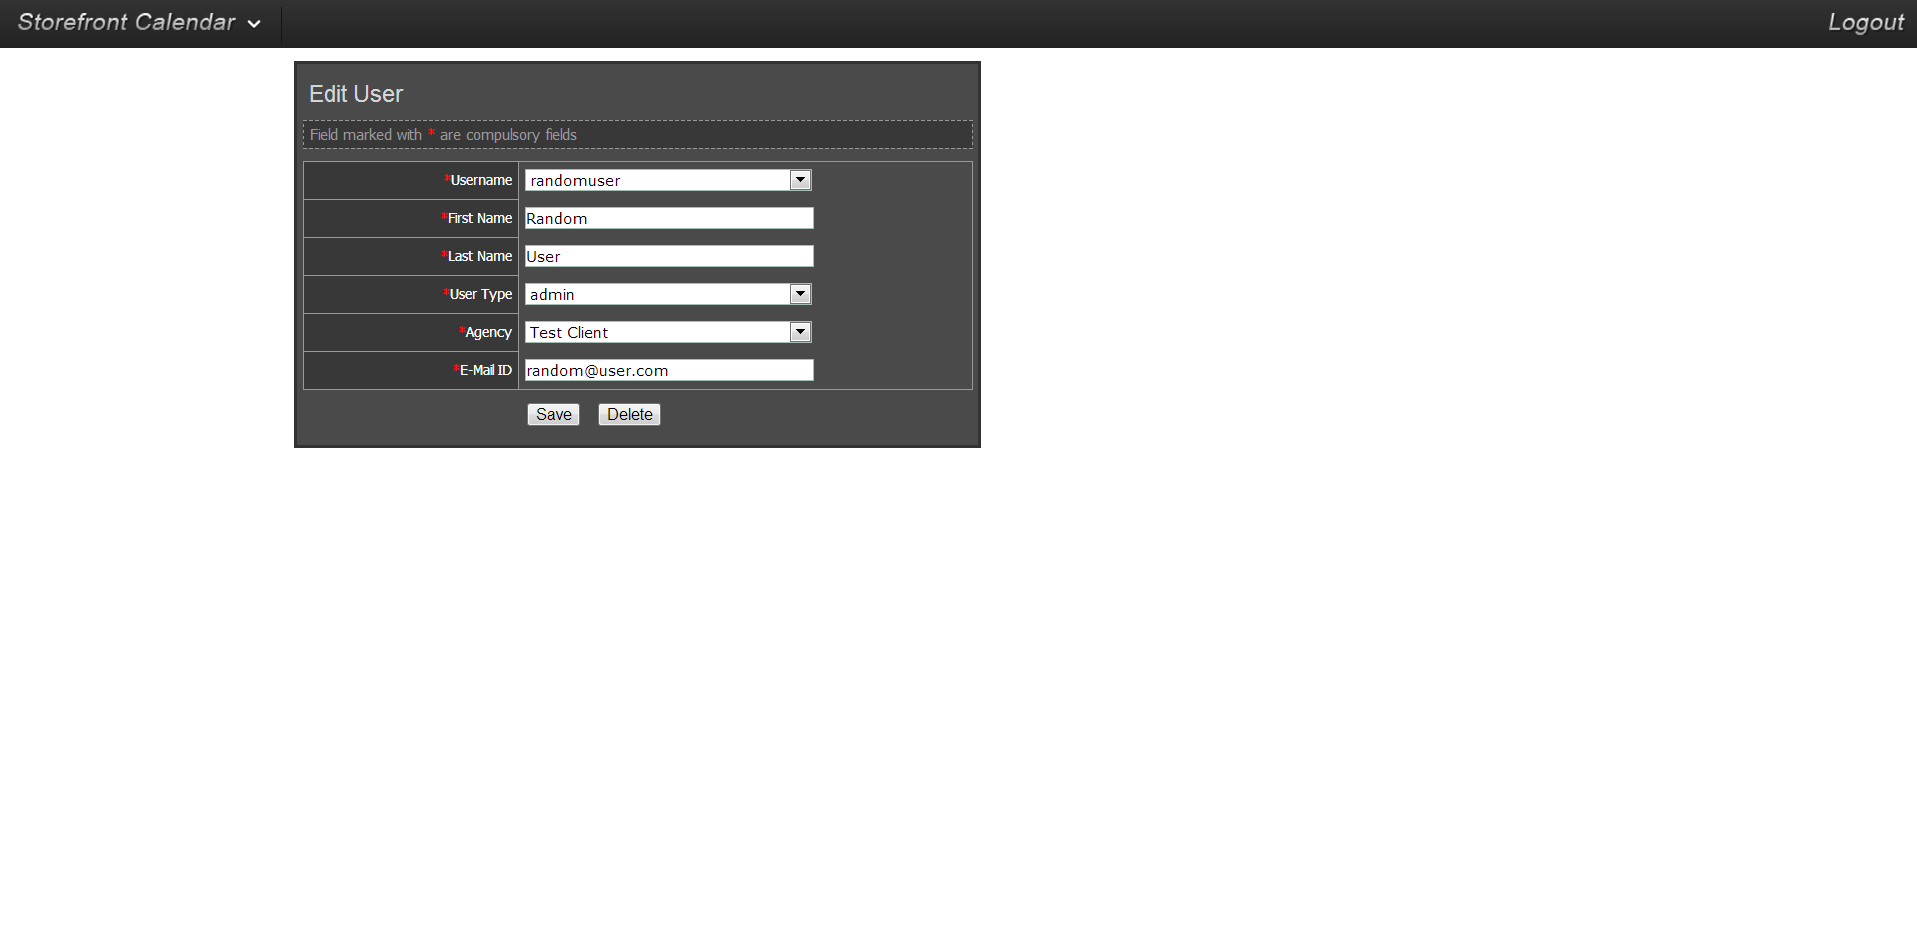
\includegraphics[width=\linewidth]{screenshots/img_edituser}



        \newpage
\section{Adding and Editing Clients/Partners (Administrators Only)}

Only Administrators can add and edit Storefront Partners (Clients).


\subsection{Adding a New Storefront Partner}

To add a new Storefront Partner to the system, select ``Add New Client'' from the drop-down menu in the Toolbar. You will be directed to the ``Add New Client'' form. Fill out all the required fields in the form, and click ``Continue''. If you want to clear the form, click 'Reset'.

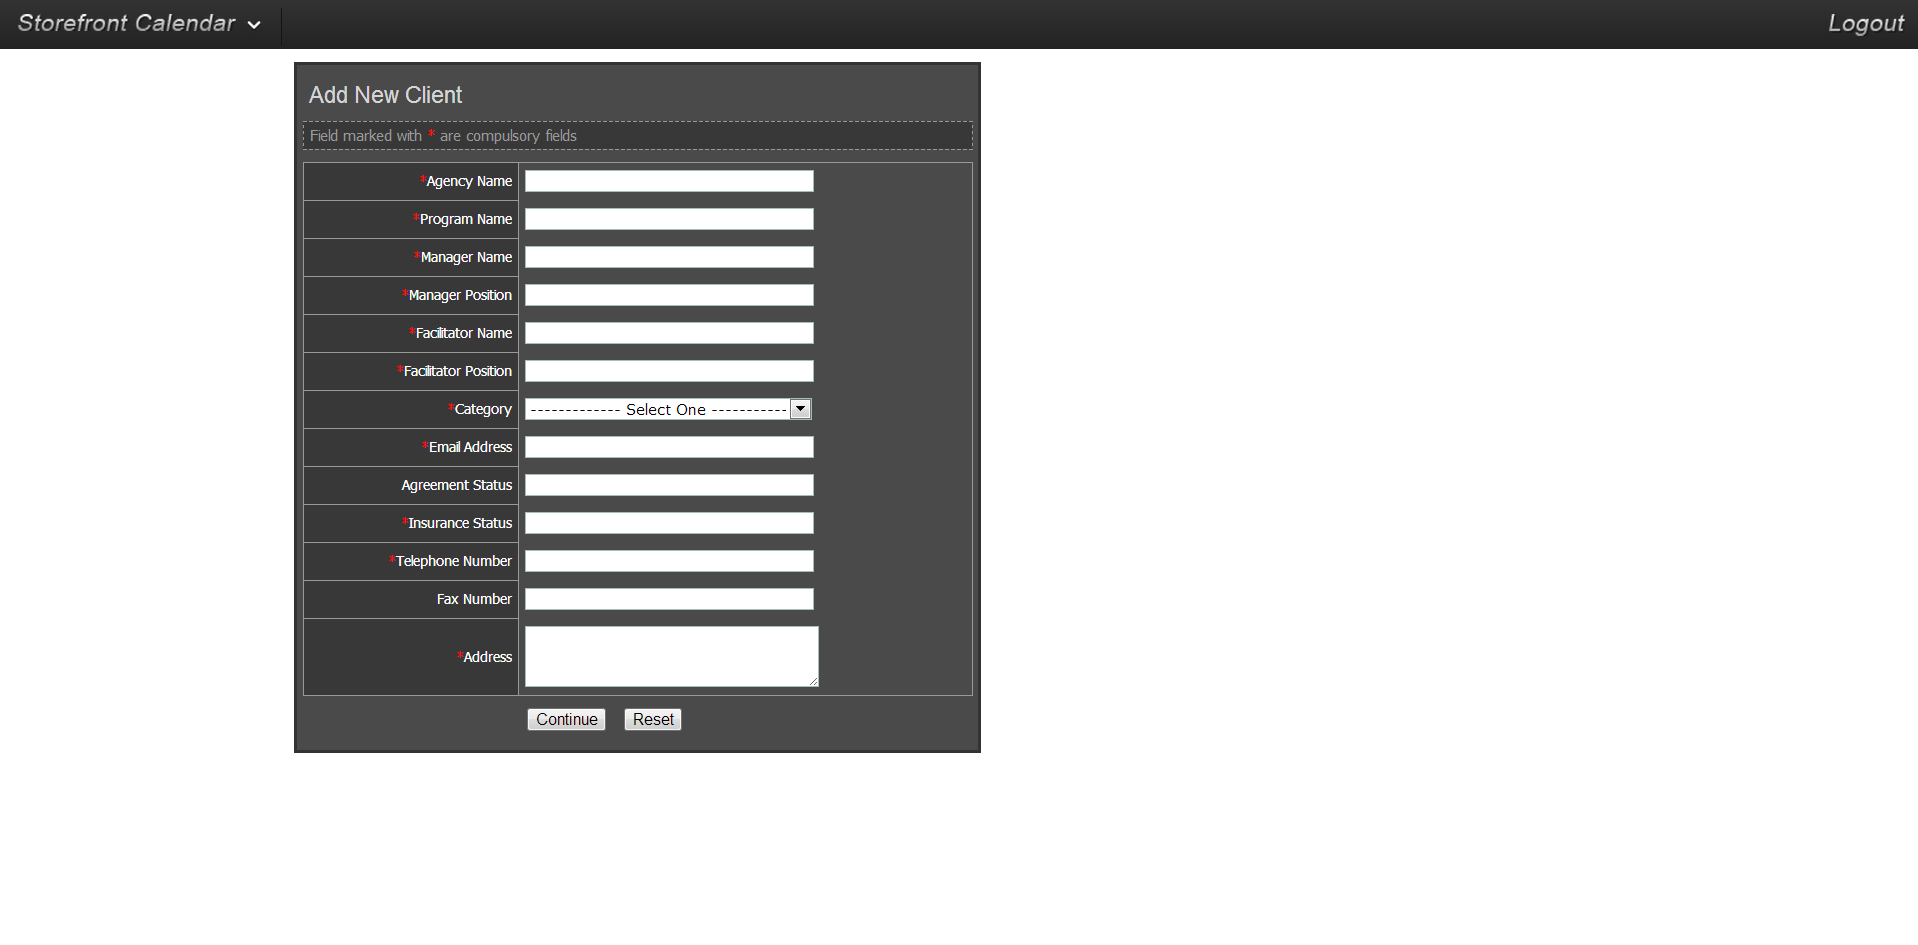
\includegraphics[width=\linewidth]{screenshots/img_addclient}


\newpage


\subsection{Editing an Existing Storefront Partner}

To edit an existing Storefront Partner, select ``Edit Client'' from the drop-down menu in the Toolbar. You will be directed to the ``Edit Client'' form. Fill out all the required fields in the form, and click ``Save''. If you want to delete the Partner, click ``Delete''.

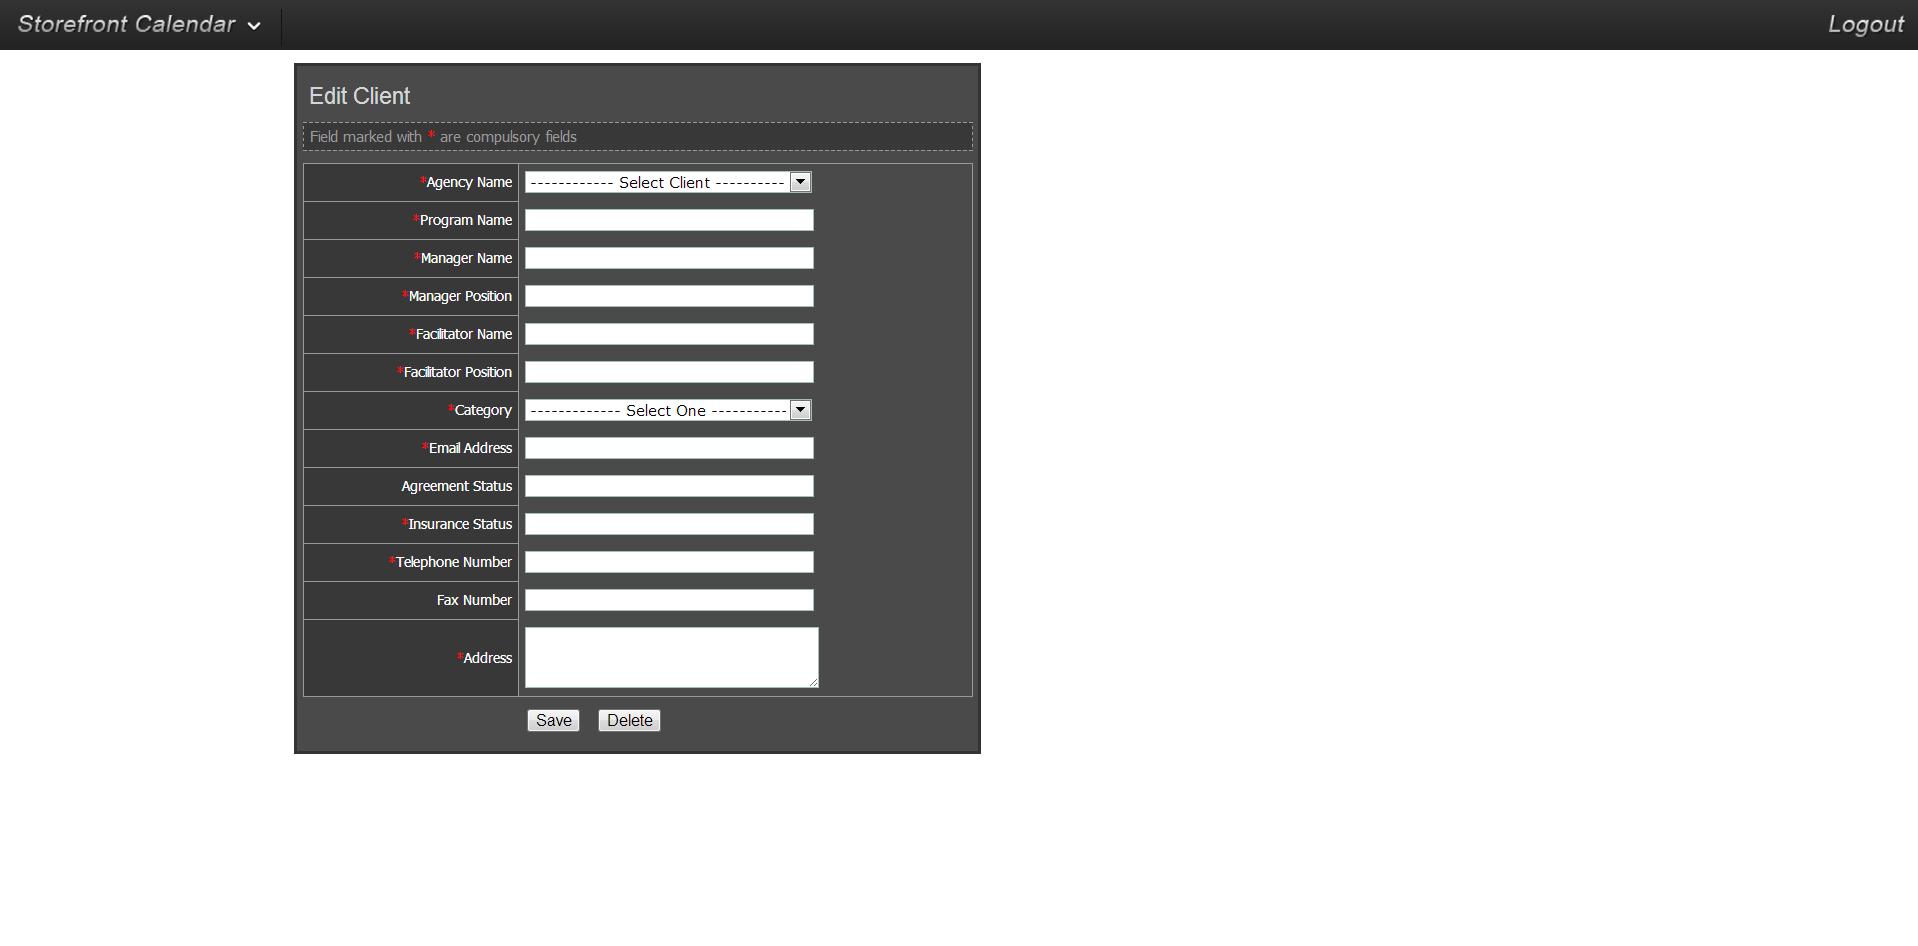
\includegraphics[width=\linewidth]{screenshots/img_editclient}




      \newpage
\section{Miscellaneous Features}


\subsection{Viewing a Map of Bookable Storefront Spaces}

To view a map of the Storefront facilities, select ``Rooms'' from the drop-down menu in the Toolbar. You will be directed to a map-view of the Storefront. Rooms outlined in green are bookable through the Calendar system. Hover over a room to see its details, including its capacity and any notes made about it.

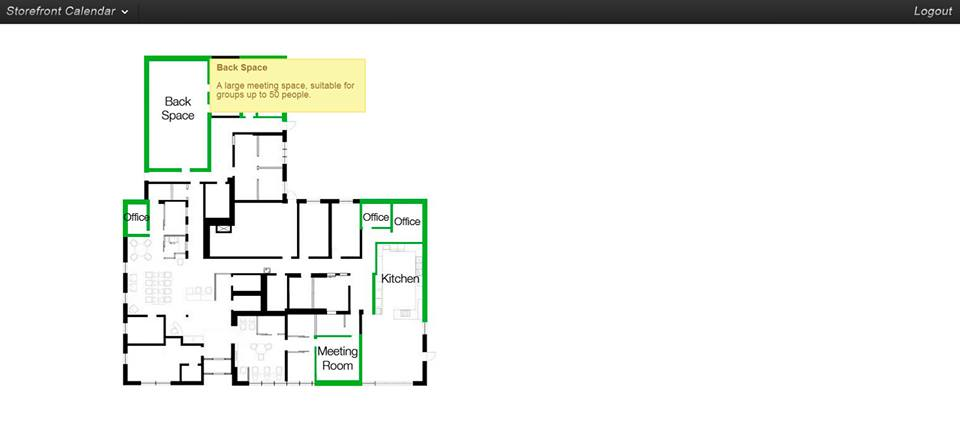
\includegraphics[width=\linewidth]{screenshots/img_map}

\newpage


\subsection{Changing Your Password}

To change your password, select ``Update Password'' from the drop-down menu in the Toolbar. You will be directed to the ``Update Password'' form. Fill out all the required fields in the form, and click ``Change Password''.

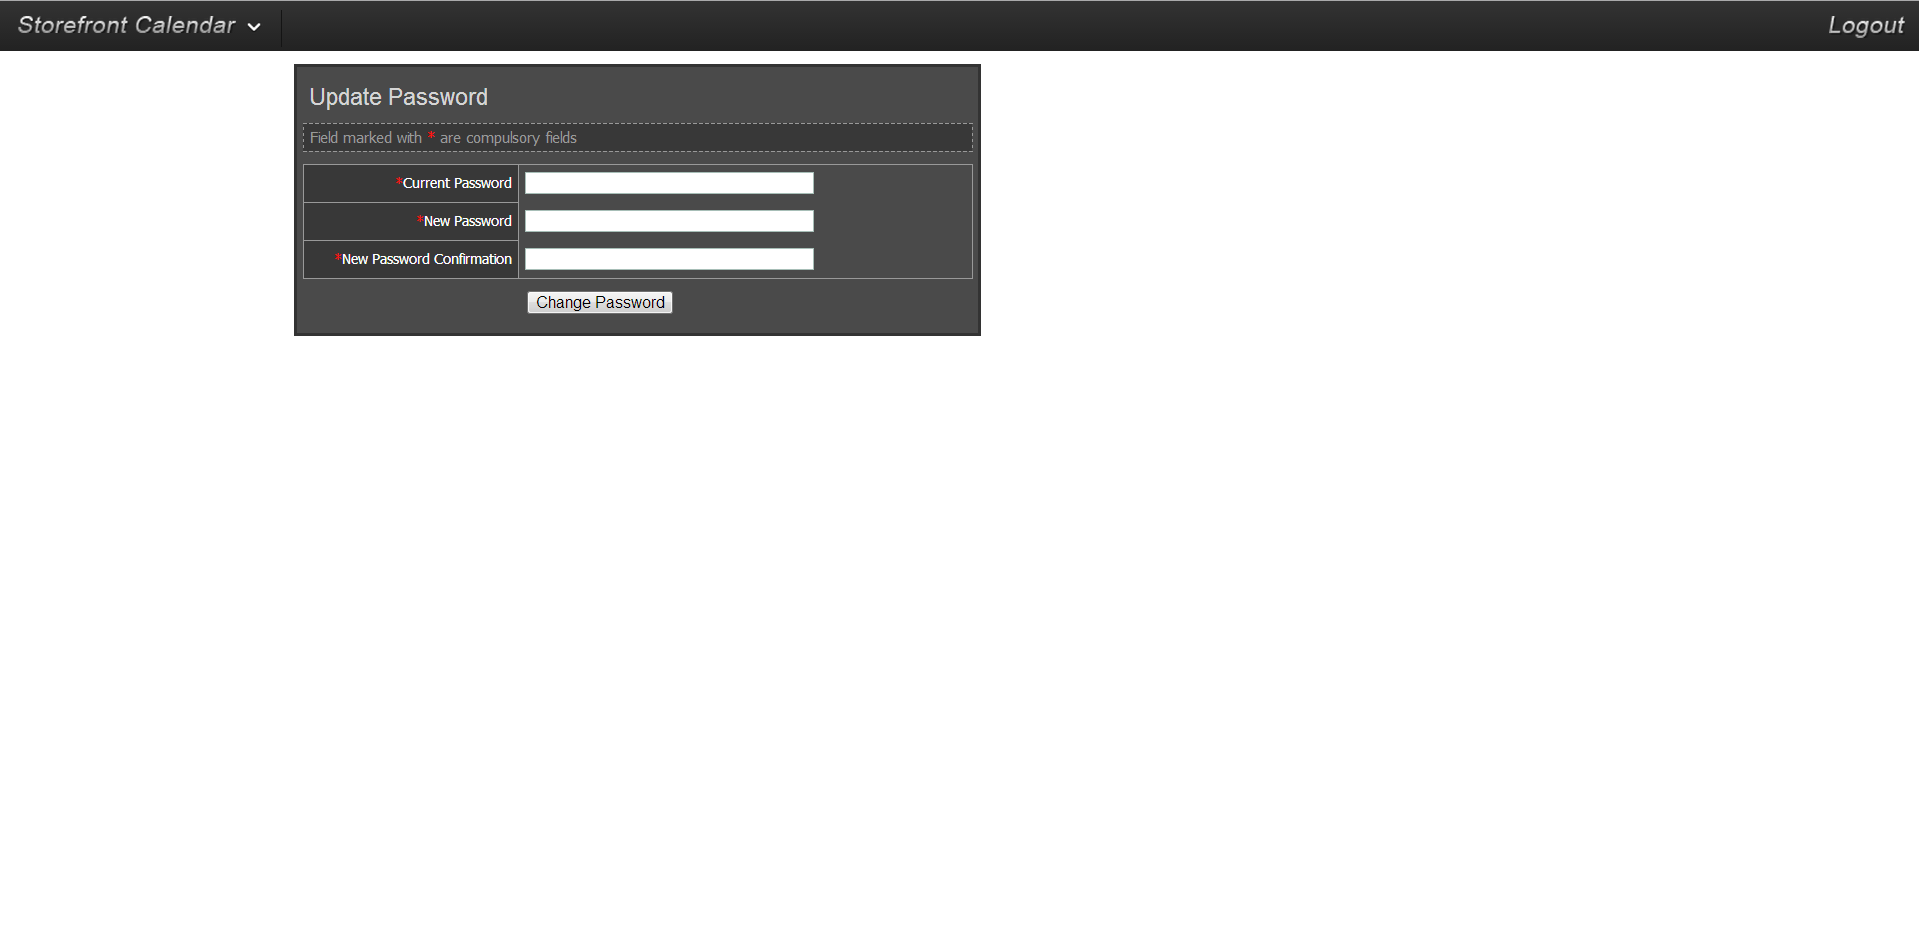
\includegraphics[width=\linewidth]{screenshots/img_password}

\newpage


\subsection{Forgot Your Password?}

In the event you have forgotten your password, click the ``Forgot Password'' link in the ``LOGIN'' box. You will be redirected to a page where you can enter your email address. You will be emailed a new, temporary password, which you should change as soon as possible.

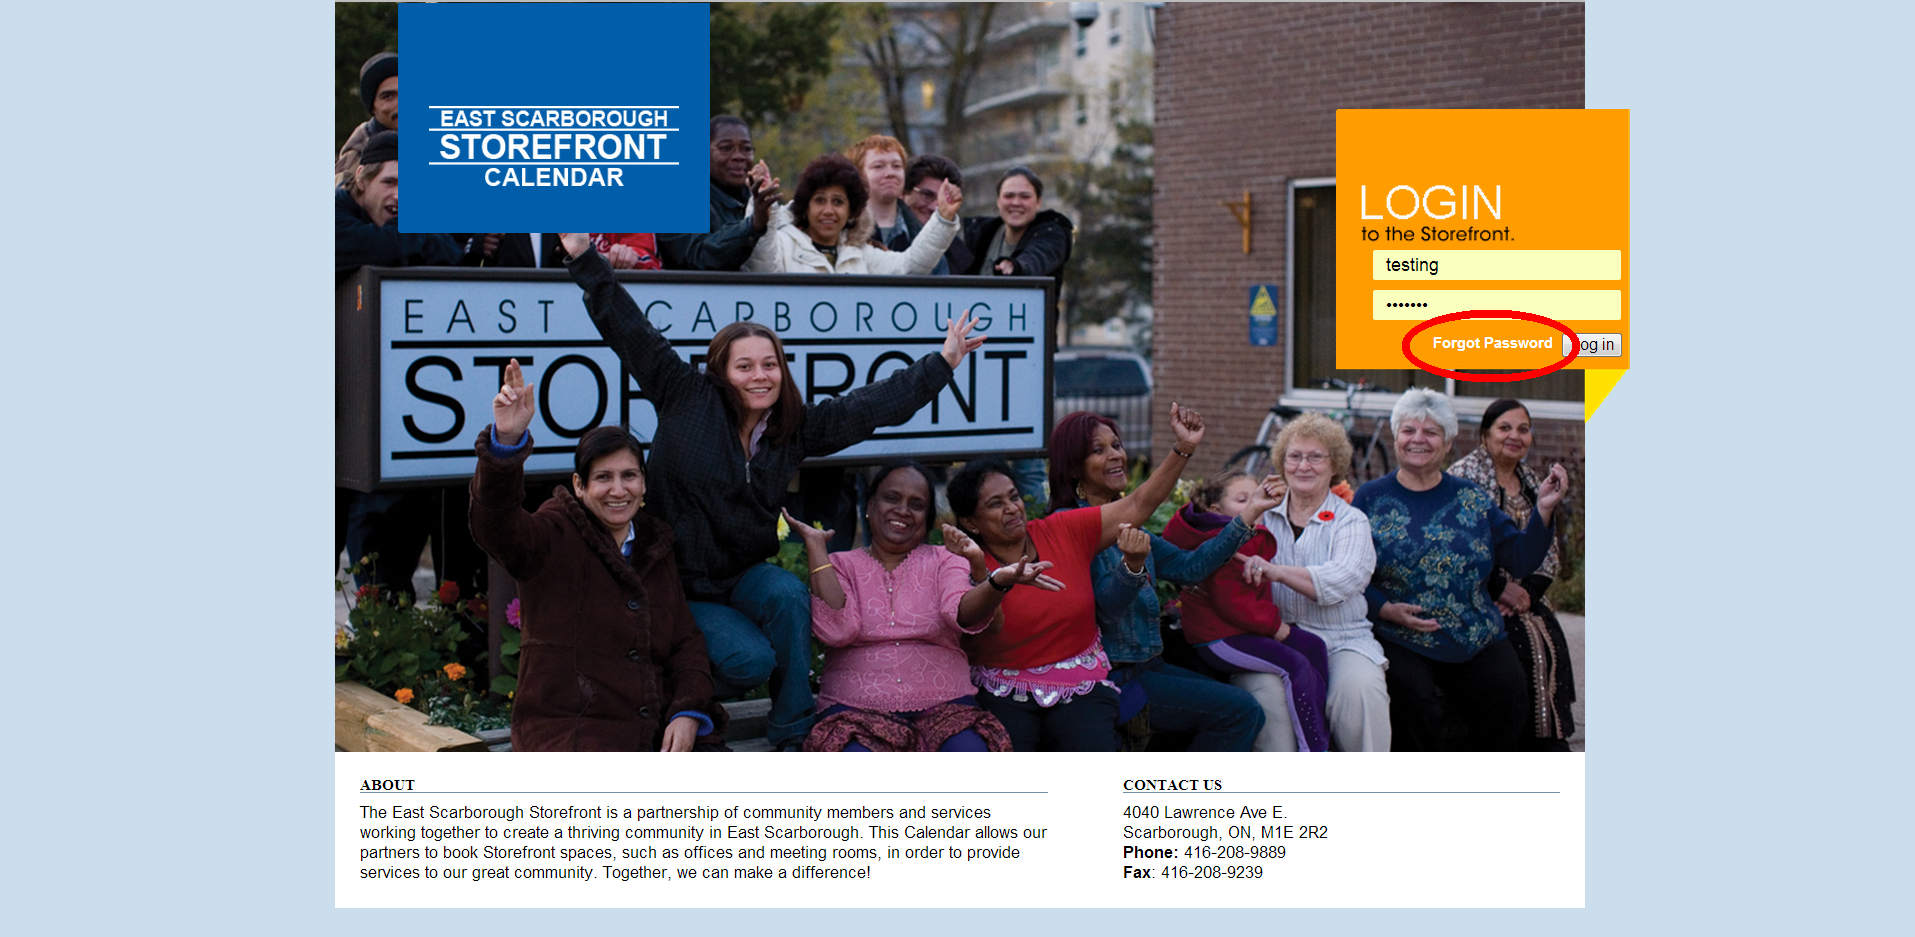
\includegraphics[width=\linewidth]{screenshots/img_forgotpass}


         \newpage

\end{document}

